% Time course of events in an experiment
% Author: Rudolf Siegel
\documentclass[tikz,border=10pt]{standalone}
\usetikzlibrary{positioning}
\usetikzlibrary{trees, shapes,shadows,shadows.blur}
\usetikzlibrary{chains,shapes.arrows,fit}
\usetikzlibrary{snakes}
\usepackage{tikz,stackengine}
\usetikzlibrary{tikzmark,fit,backgrounds,mindmap,decorations.text,shapes.callouts,arrows}
\usetikzlibrary{arrows, chains,through, positioning, trees, shapes.symbols}
\usetikzlibrary{shadings,positioning}
\usetikzlibrary{arrows,automata}
\usetikzlibrary{optics, arrows.meta}
\usetikzlibrary{decorations.markings, fpu, decorations.pathreplacing, decorations.text, decorations.footprints, calc}

\begin{document}
	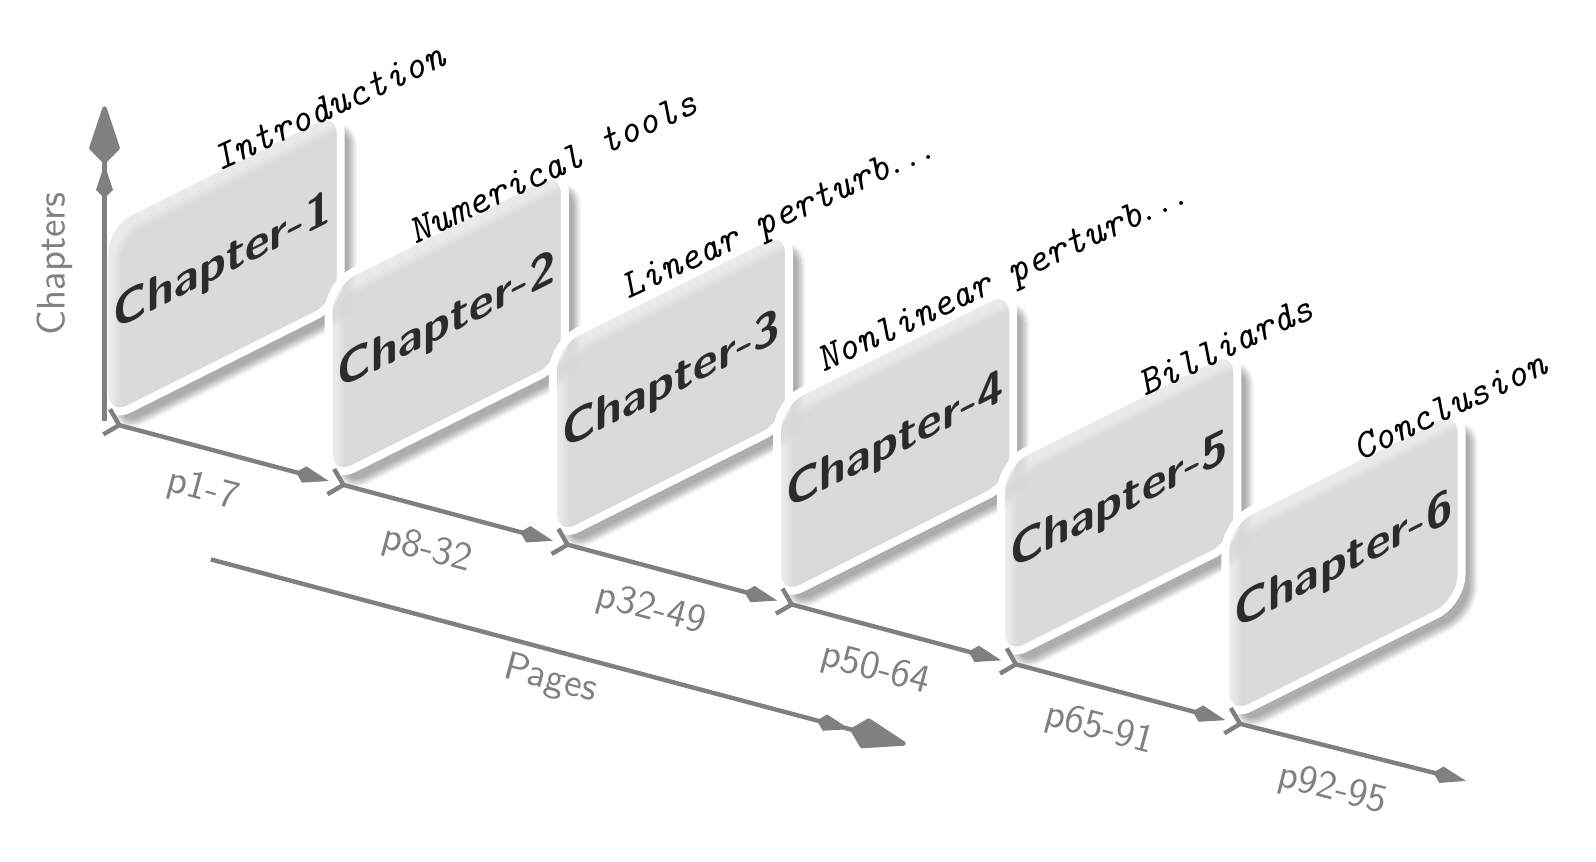
\begin{tikzpicture}
			\tikzset{scale=0.27,
					basefont/.style = {font = \Large\sffamily},
					timing/.style = {basefont, sloped,},
					label/.style = {basefont, align = left,},
					screen/.style = {basefont, black, align = center,	minimum size = 2.5cm, fill = gray!20, draw = white, fill opacity=0.8, line width=1mm,
						blur shadow={shadow blur steps=10,
									shadow blur extra rounding=10pt, 
									shadow xshift=1ex,
									shadow yshift=-1ex},
						rounded corners=10,
					%	shading=ball,
					%	ball color=white
					}};
			
			% macro for defining screens
			\newcommand*{\screen}[4]{%
					\begin{scope}[xshift  =#3, yshift = #4,
							every node/.append style = {yslant = 0.5},
							yslant = 0.33,
							local bounding box = #1]
							\node[screen] at (4cm,4cm) {#2};
						\end{scope}
				} 	
			% define several screens
			\screen{frame1}{\LARGE\textbf{Chapter-1}}{0}  {0}
			\screen{frame2}{\LARGE\textbf{Chapter-2}}{300}{-80}
			\screen{frame3}{\LARGE\textbf{Chapter-3}}{600}{-160}
			\screen{frame4}{\LARGE\textbf{Chapter-4}}{900}{-240}
			\screen{frame5}{\LARGE\textbf{Chapter-5}}{1200}{-320}
			\screen{frame6}{\LARGE\textbf{Chapter-6}}{1500}{-400};
%			\screen{frame7}{.}{1800}{-480};
			\coordinate[xshift=480, yshift=-146] (frame7);
%			\coordinate[xshift=390, yshift=-57.5] (frame8);
			
			% add annotations
			\foreach \i / \content in {
					1/\textit{\texttt{Introduction}},
					2/\textit{\texttt{Numerical tools}},
					3/\textit{\texttt{Linear perturb$\ldots$}},
					4/\textit{\texttt{Nonlinear perturb$\ldots$}},
					5/\textit{\texttt{Billiards}},
					6/\textit{\texttt{Conclusion}}%\\(depending on response)
%					7/\textit{\texttt{Bibliography}}%\\(depending on response)
				}
			\node[label, rotate=25, above=5em and 5em of frame\i.east]
			(f\i-label) {\content};
			
%			
			% add time course
			\foreach \j [count=\i] / \content in {
					2/p1-7\,,
					3/p8-32\,,
					4/p32-49\,,
					5/p50-64\,,
					6/p65-91\,,
					7/p92-95\,
				}
			\path[ultra thick, gray, arrows = {Straight Barb[reversed]-Kite[]}] (frame\i.south west) edge 	node[timing, below=0.5em] {\content} (frame\j.south west);
			
			% some manual addition
			\path[ultra thick, gray, arrows = {-Kite[]Kite[length=8mm, round,  gray]}] (frame1.south west) ++(5,-6.5) edge node[timing, below] {Pages} ([xshift=5mm,yshift=-6.75cm]frame4.south);
			\path[ultra thick, gray, arrows = {-Kite[]Kite[length=8mm, round,  gray]}] (frame1.south west) edge node[timing, above=0.75em] {Chapters} (frame1.north west);
		\end{tikzpicture}
\end{document}